

\section{Resultados}

Se explicaran ahora los resultados que hemos obtenido usando todos los recursos explicados anteriormente:

\subsection{Human Phenotipe Ontology}

\hfill

Tras realizar una búsqueda del fenotipo a investigar, \textit{Dyscalculia}, vemos que se encuentra clasificado como \href{https://hpo.jax.org/app/browse/term/HP:0002442}{HP:0002442} con un total de 13 fenotipos de otras enfermedades asociadas y un total de 24 genes asociados a esta en HPO.

Descargamos un .csv para cargar el listado de genes con sus links en String

\subsection{String}

\hfill

Gracias a las anotaciones en HPO obtenidas del .csv mencionado anteriormente, podemos obtener los genes asociados del fenotipo, y con ello procedemos a la búsqueda de más información acerca de estos utilizando \href{https://string-db.org}{STRING}, una base de datos biológica y un recurso web de interacciones entre proteínas. El resultado lo podemos ver en la figura 1

\begin{figure}[h]
	\centering
	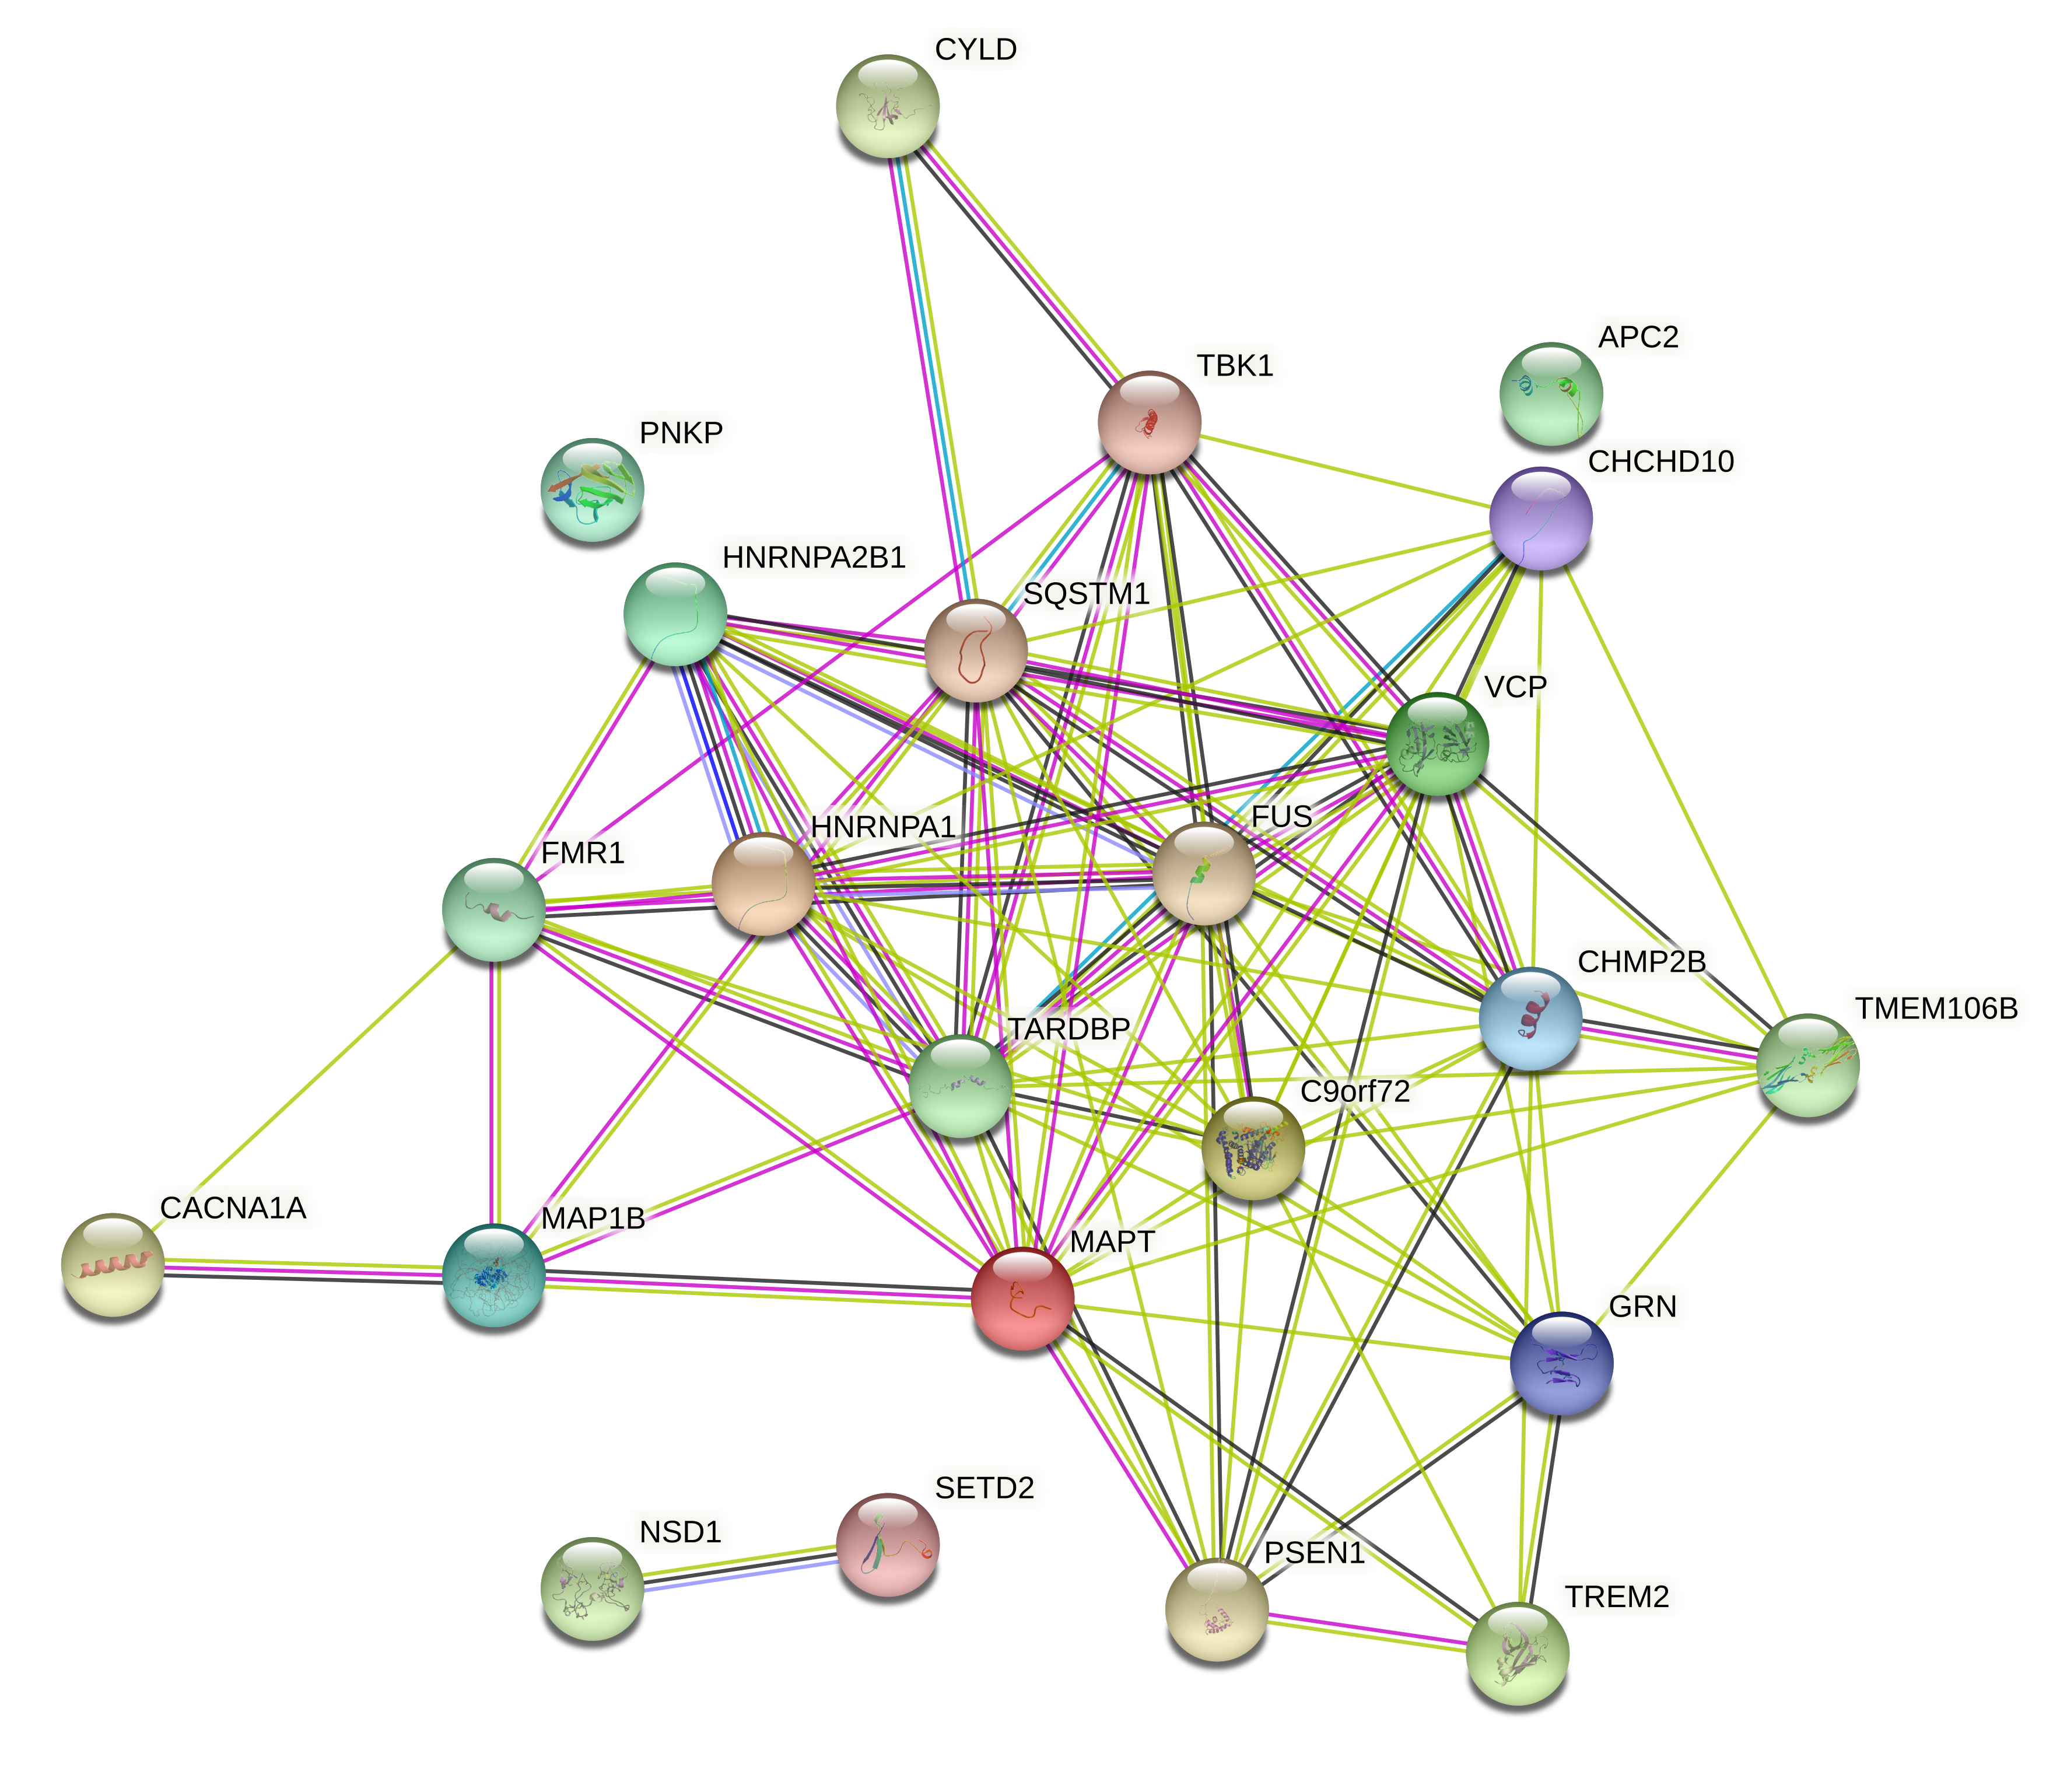
\includegraphics[width=0.90\textwidth]{figures/Gene_Relationship.png}
	\caption{Interacciones proteína-proteína a raíz de los genes relacionados. }
	\label{fig:string1}
\end{figure}

Una vez cargados los genes y sus relaciones en string, procedemos a descargar los ficheros "string-node-degree.tsv" e "string-interactions.tsv".

Se creara también un objeto network de la librería de R stringdb, con las siguientes caracteristicas:

Versión=11
Specie=9606
Score threshold=400

\hfill

Se usara esta network de genes humanos, para buscar genes vecinos de los 24 que teníamos en un principio y realizar una propagación de red con el fin de aumentar el total de genes a estudiar que guarden directa o indirectamente una relación con nuestro fenotipo a estudiar.

\hfill

Gracias a este método el total de genes de estudio ha ascendido a 214, con esto podemos pasar al estudio de sus relaciones y funciones con una carga de trabajo mas adecuada.

Finalmente se usara String para la documentación que estudiaremos antes de sacar conclusiones, puesta herramienta nos sugiere papers científicos de gran relación con la red de genes que se le de como entrada

\subsection{igraph}

Usaremos igraph para convertir nuestro objeto network (genes originalmente relacionados con el  fenotipo mas los genes vecinos de la red general anteriormente citada) en un dataframe que sea procesable por las funciones de clustering para la división en comunidades

\hfill

\subsection{Análisis por comunidades}

Se realizan a continuación los correspondientes pasos para clusterizar nuestro conjunto en distintas comunidades y realizar el correspondiente análisis de enriquecimiento funcional a las adecuadas:

\subsubsection{LinkComm}

Tras una serie de pruebas con distintas funciones de igraph para hacer comunidades, se ha decidido usar la anteriormente citada LinkComm (con hcmethod="single", ya que cambiando este parametro a otros modos como "ward, obteniamos comunidades mucho menos relevantes), que nos deja la figura 2 como muestra de su trabajo sobre nuestra red de genes, este dendograma y esta gráfica que relaciona la altura con la densidad de partición :

\begin{figure}[h]
	\centering
	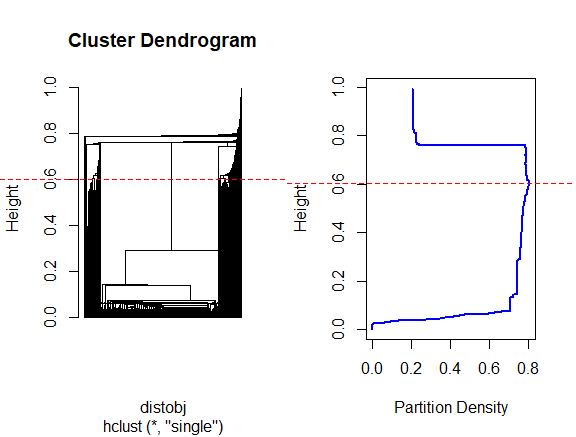
\includegraphics[width=0.60\textwidth]{figures/Grapichs_LinkComm.png}
	\caption{Dendograma del clustering realizado-Relación Altura con Densidad de particion. }
	\label{fig:LinkComm1}
\end{figure}

\newpage

\hfill

Se han obtenido un total de 71 comunidades, cada una con una cantidad de los 214 nodos originales diferente. Observamos en esta con un gráfico de barras la cantidad de nodos que tienen esas comunidades:

\begin{figure}[h]
	\centering
	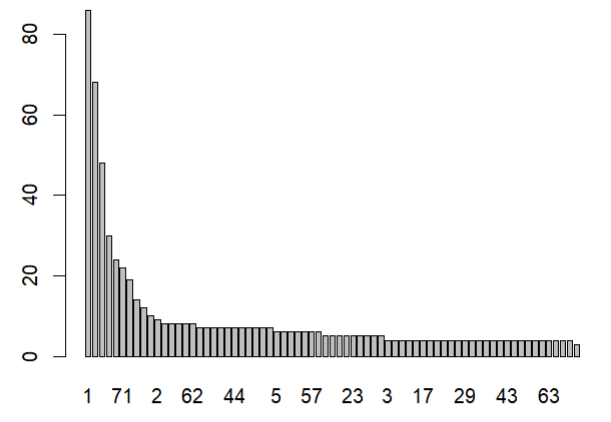
\includegraphics[width=0.70\textwidth]{figures/barplot_communities.PNG}
	\caption{Cantidad de genes de cada comunidad obtenida.}
	\label{fig:LinkComm2}
\end{figure}


Además podemos observar esta imagen en la que por colores se nos muestra la pertenencia de cada nodo de la red a la una comunidad u otra:

\begin{figure}[h]
	\centering
	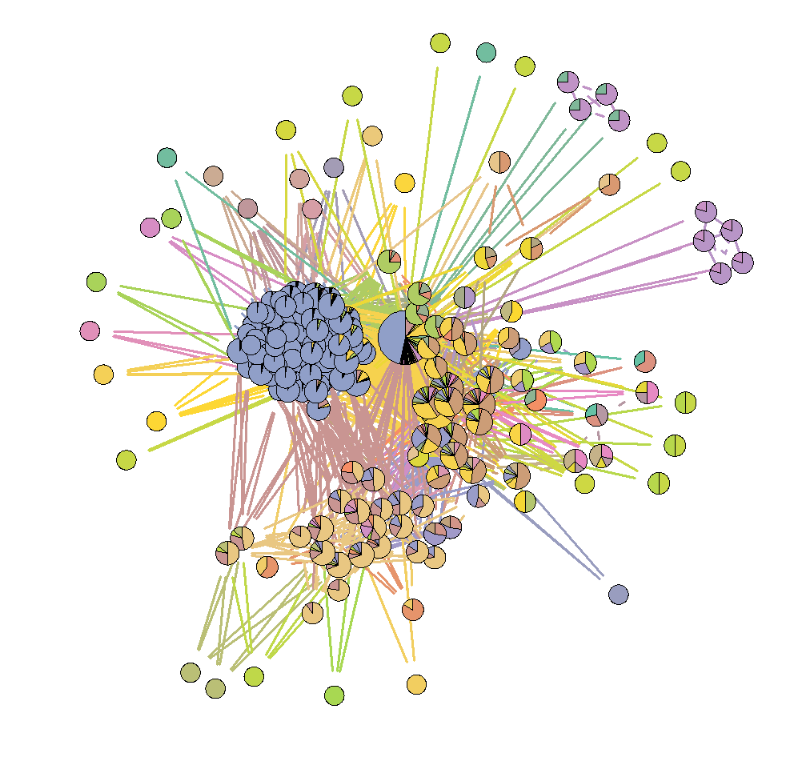
\includegraphics[width=0.65\textwidth]{figures/Grafo_Linkcomm.PNG}
	\caption{Pertenencia a las distintas comunidades de nuestra red de genes. }
	\label{fig:LinkComm3}
\end{figure}



\subsection{ClusterProfiler}

A continuación se realizara un enriquecimiento funcional con GO (Gene Ontology) para observar las funciones implicadas en la formación de las distintas componentes celulares de las principales comunidades que hemos obtenido con LinkComm.

\hfill

\textbf{Enriquecimiento genes originales}

24 Genes originales

\hfill

\begin{table}[ht]
\centering
\begin{tabular}{rlll}
  \hline
 & ID & Description & GeneRatio \\ 
  \hline
1 & GO:0031305 & integral component of mitochondrial inner membrane & 1/1 \\ 
  2 & GO:0031304 & intrinsic component of mitochondrial inner membrane & 1/1 \\ 
  3 & GO:0005758 & mitochondrial intermembrane space & 1/1 \\ 
  4 & GO:0032592 & integral component of mitochondrial membrane & 1/1 \\ 
  5 & GO:0031970 & organelle envelope lumen & 1/1 \\ 
  6 & GO:0098573 & intrinsic component of mitochondrial membrane & 1/1 \\ 
  7 & GO:0098800 & inner mitochondrial membrane protein complex & 1/1 \\ 
  8 & GO:0098798 & mitochondrial protein-containing complex & 1/1 \\ 
  9 & GO:0031301 & integral component of organelle membrane & 1/1 \\ 
  10 & GO:0031300 & intrinsic component of organelle membrane & 1/1 \\ 
   \hline
\end{tabular}
\end{table}

\begin{table}[ht]
\centering
\begin{tabular}{rllrrlr}
  \hline
 & ID & BgRatio & pvalue & p.adjust & geneID & Count \\ 
  \hline
1 & GO:0031305 & 60/19869 & 0.00 & 0.01 & CHCHD10 &   1 \\ 
  2 & GO:0031304 & 61/19869 & 0.00 & 0.01 & CHCHD10 &   1 \\ 
  3 & GO:0005758 & 84/19869 & 0.00 & 0.01 & CHCHD10 &   1 \\ 
  4 & GO:0032592 & 92/19869 & 0.00 & 0.01 & CHCHD10 &   1 \\ 
  5 & GO:0031970 & 94/19869 & 0.00 & 0.01 & CHCHD10 &   1 \\ 
  6 & GO:0098573 & 94/19869 & 0.00 & 0.01 & CHCHD10 &   1 \\ 
  7 & GO:0098800 & 158/19869 & 0.01 & 0.01 & CHCHD10 &   1 \\ 
  8 & GO:0098798 & 295/19869 & 0.01 & 0.02 & CHCHD10 &   1 \\ 
  9 & GO:0031301 & 390/19869 & 0.02 & 0.02 & CHCHD10 &   1 \\ 
  10 & GO:0031300 & 420/19869 & 0.02 & 0.02 & CHCHD10 &   1 \\ 
   \hline
\end{tabular}
\end{table}

\newpage

\textbf{Enrich Comm 64}

Comunidad 64 con 68 genes

\hfill

\begin{table}[ht]
\centering
\begin{tabular}{rlll}
  \hline
 & ID & Description & GeneRatio \\ 
  \hline
1 & GO:0035578 & azurophil granule lumen & 12/18 \\ 
  2 & GO:0005766 & primary lysosome & 12/18 \\ 
  3 & GO:0042582 & azurophil granule & 12/18 \\ 
  4 & GO:0005775 & vacuolar lumen & 12/18 \\ 
  5 & GO:0034774 & secretory granule lumen & 13/18 \\ 
  6 & GO:0060205 & cytoplasmic vesicle lumen & 13/18 \\ 
  7 & GO:0031983 & vesicle lumen & 13/18 \\ 
  8 & GO:0035580 & specific granule lumen & 5/18 \\ 
  9 & GO:0042581 & specific granule & 5/18 \\ 
  10 & GO:0062023 & collagen-containing extracellular matrix & 4/18 \\
   \hline
\end{tabular}
\end{table}

\begin{table}[ht]
\centering
\begin{tabular}{rllrrr}
  \hline
 & ID & BgRatio & pvalue & p.adjust & Count \\ 
  \hline
1 & GO:0035578 & 91/19869 & 0.00 & 0.00 &  12 \\ 
  2 & GO:0005766 & 155/19869 & 0.00 & 0.00 &  12 \\ 
  3 & GO:0042582 & 155/19869 & 0.00 & 0.00 &  12 \\ 
  4 & GO:0005775 & 176/19869 & 0.00 & 0.00 &  12 \\ 
  5 & GO:0034774 & 322/19869 & 0.00 & 0.00 &  13 \\ 
  6 & GO:0060205 & 325/19869 & 0.00 & 0.00 &  13 \\ 
  7 & GO:0031983 & 327/19869 & 0.00 & 0.00 &  13 \\ 
  8 & GO:0035580 & 62/19869 & 0.00 & 0.00 &   5 \\ 
  9 & GO:0042581 & 160/19869 & 0.00 & 0.00 &   5 \\ 
  10 & GO:0062023 & 433/19869 & 0.00 & 0.00 &   4 \\
   \hline
\end{tabular}
\end{table}

\begin{table}[ht]
\centering
\begin{tabular}{rll}
  \hline
 & ID & geneID \\ 
  \hline
1 & GO:0035578 & RETN/MPO/LYZ/AGA/CTSG/RNASE3/S100A7/ORM2/ELANE/PRDX6/TXNDC5/FRK \\ 
  2 & GO:0005766 & RETN/MPO/LYZ/AGA/CTSG/RNASE3/S100A7/ORM2/ELANE/PRDX6/TXNDC5/FRK \\ 
  3 & GO:0042582 & RETN/MPO/LYZ/AGA/CTSG/RNASE3/S100A7/ORM2/ELANE/PRDX6/TXNDC5/FRK \\ 
  4 & GO:0005775 & RETN/MPO/LYZ/AGA/CTSG/RNASE3/S100A7/ORM2/ELANE/PRDX6/TXNDC5/FRK \\ 
  5 & GO:0034774 & RETN/MPO/LYZ/AGA/CTSG/RNASE3/S100A7/ORM2/INS/ELANE/PRDX6/TXNDC5/FRK \\ 
  6 & GO:0060205 & RETN/MPO/LYZ/AGA/CTSG/RNASE3/S100A7/ORM2/INS/ELANE/PRDX6/TXNDC5/FRK \\ 
  7 & GO:0031983 & RETN/MPO/LYZ/AGA/CTSG/RNASE3/S100A7/ORM2/INS/ELANE/PRDX6/TXNDC5/FRK \\ 
  8 & GO:0035580 & RETN/LYZ/ORM2/ELANE/FRK \\ 
  9 & GO:0042581 & RETN/LYZ/ORM2/ELANE/FRK \\ 
  10 & GO:0062023 & CTSG/S100A7/ORM2/ELANE \\ 
   \hline
\end{tabular}
\end{table}

\newpage

\textbf{Comunidad 70}

Comunidad 70 con 48 genes

\hfill

\begin{table}[ht]
\centering
\begin{tabular}{rlll}
  \hline
 & ID & Description & GeneRatio \\ 
  \hline
1 & GO:0035578 & azurophil granule lumen & 6/8 \\ 
  2 & GO:0005766 & primary lysosome & 6/8 \\ 
  3 & GO:0042582 & azurophil granule & 6/8 \\ 
  4 & GO:0005775 & vacuolar lumen & 6/8 \\ 
  5 & GO:0034774 & secretory granule lumen & 6/8 \\ 
  6 & GO:0060205 & cytoplasmic vesicle lumen & 6/8 \\ 
  7 & GO:0031983 & vesicle lumen & 6/8 \\ 
  8 & GO:0045335 & phagocytic vesicle & 2/8 \\ 
  9 & GO:0030139 & endocytic vesicle & 2/8 \\ 
  10 & GO:0071682 & endocytic vesicle lumen & 1/8 \\ 
   \hline
\end{tabular}
\end{table}

\begin{table}[ht]
\centering
\begin{tabular}{rllrrr}
  \hline
 & ID & BgRatio & pvalue & p.adjust & Count \\ 
  \hline
1 & GO:0035578 & 91/19869 & 0.00 & 0.00 &   6 \\ 
  2 & GO:0005766 & 155/19869 & 0.00 & 0.00 &   6 \\ 
  3 & GO:0042582 & 155/19869 & 0.00 & 0.00 &   6 \\ 
  4 & GO:0005775 & 176/19869 & 0.00 & 0.00 &   6 \\ 
  5 & GO:0034774 & 322/19869 & 0.00 & 0.00 &   6 \\ 
  6 & GO:0060205 & 325/19869 & 0.00 & 0.00 &   6 \\ 
  7 & GO:0031983 & 327/19869 & 0.00 & 0.00 &   6 \\ 
  8 & GO:0045335 & 139/19869 & 0.00 & 0.00 &   2 \\ 
  9 & GO:0030139 & 343/19869 & 0.01 & 0.03 &   2 \\ 
  10 & GO:0071682 & 23/19869 & 0.01 & 0.03 &   1 \\ 
   \hline
\end{tabular}
\end{table}

\begin{table}[ht]
\centering
\begin{tabular}{rll}
  \hline
 & ID & geneID \\ 
  \hline
1 & GO:0035578 & MPO/RNASE3/RNASE2/TUBB4B/PRDX6/ELANE \\ 
  2 & GO:0005766 & MPO/RNASE3/RNASE2/TUBB4B/PRDX6/ELANE \\ 
  3 & GO:0042582 & MPO/RNASE3/RNASE2/TUBB4B/PRDX6/ELANE \\ 
  4 & GO:0005775 & MPO/RNASE3/RNASE2/TUBB4B/PRDX6/ELANE \\ 
  5 & GO:0034774 & MPO/RNASE3/RNASE2/TUBB4B/PRDX6/ELANE \\ 
  6 & GO:0060205 & MPO/RNASE3/RNASE2/TUBB4B/PRDX6/ELANE \\ 
  7 & GO:0031983 & MPO/RNASE3/RNASE2/TUBB4B/PRDX6/ELANE \\ 
  8 & GO:0045335 & MPO/ELANE \\ 
  9 & GO:0030139 & MPO/ELANE \\ 
  10 & GO:0071682 & MPO \\
   \hline
\end{tabular}
\end{table}

\newpage

\textbf{Comunidad 33}

Comunidad 33 con 30 genes

\hfill

\begin{table}[ht]
\centering
\begin{tabular}{rlll}
  \hline
 & ID & Description & GeneRatio \\ 
  \hline
1 & GO:0035578 & azurophil granule lumen & 9/10 \\ 
  2 & GO:0005766 & primary lysosome & 9/10 \\ 
  3 & GO:0042582 & azurophil granule & 9/10 \\ 
  4 & GO:0034774 & secretory granule lumen & 10/10 \\ 
  5 & GO:0060205 & cytoplasmic vesicle lumen & 10/10 \\ 
  6 & GO:0031983 & vesicle lumen & 10/10 \\ 
  7 & GO:0005775 & vacuolar lumen & 9/10 \\ 
  8 & GO:0035580 & specific granule lumen & 6/10 \\ 
  9 & GO:0042581 & specific granule & 6/10 \\ 
  10 & GO:0062023 & collagen-containing extracellular matrix & 5/10 \\ 
   \hline
\end{tabular}
\end{table}

\begin{table}[ht]
\centering
\begin{tabular}{rllrrr}
  \hline
 & ID & BgRatio & pvalue & p.adjust & Count \\ 
  \hline
1 & GO:0035578 & 91/19869 & 0.00 & 0.00 &   9 \\ 
  2 & GO:0005766 & 155/19869 & 0.00 & 0.00 &   9 \\ 
  3 & GO:0042582 & 155/19869 & 0.00 & 0.00 &   9 \\ 
  4 & GO:0034774 & 322/19869 & 0.00 & 0.00 &  10 \\ 
  5 & GO:0060205 & 325/19869 & 0.00 & 0.00 &  10 \\ 
  6 & GO:0031983 & 327/19869 & 0.00 & 0.00 &  10 \\ 
  7 & GO:0005775 & 176/19869 & 0.00 & 0.00 &   9 \\ 
  8 & GO:0035580 & 62/19869 & 0.00 & 0.00 &   6 \\ 
  9 & GO:0042581 & 160/19869 & 0.00 & 0.00 &   6 \\ 
  10 & GO:0062023 & 433/19869 & 0.00 & 0.00 &   5 \\ 
   \hline
\end{tabular}
\end{table}

\begin{table}[ht]
\centering
\begin{tabular}{rll}
  \hline
 & ID & geneID \\ 
  \hline
1 & GO:0035578 & CTSG/RETN/MPO/LYZ/S100A7/TXNDC5/ORM2/ELANE/FRK \\ 
  2 & GO:0005766 & CTSG/RETN/MPO/LYZ/S100A7/TXNDC5/ORM2/ELANE/FRK \\ 
  3 & GO:0042582 & CTSG/RETN/MPO/LYZ/S100A7/TXNDC5/ORM2/ELANE/FRK \\ 
  4 & GO:0034774 & CTSG/RETN/MPO/LYZ/SLPI/S100A7/TXNDC5/ORM2/ELANE/FRK \\ 
  5 & GO:0060205 & CTSG/RETN/MPO/LYZ/SLPI/S100A7/TXNDC5/ORM2/ELANE/FRK \\ 
  6 & GO:0031983 & CTSG/RETN/MPO/LYZ/SLPI/S100A7/TXNDC5/ORM2/ELANE/FRK \\ 
  7 & GO:0005775 & CTSG/RETN/MPO/LYZ/S100A7/TXNDC5/ORM2/ELANE/FRK \\ 
  8 & GO:0035580 & RETN/LYZ/SLPI/ORM2/ELANE/FRK \\ 
  9 & GO:0042581 & RETN/LYZ/SLPI/ORM2/ELANE/FRK \\ 
  10 & GO:0062023 & CTSG/SLPI/S100A7/ORM2/ELANE \\ 
   \hline
\end{tabular}
\end{table}




\textbf{}